\setchapterpreamble[u]{\margintoc}
\chapter{Structured Output}
\label{chapter:output}

\epigraph{In limits, there is freedom. Creativity thrives within structure.}{Julia B. Cameron}

\section{Introduction}

While Language Models excel at generating human-like text, they face significant challenges when tasked with producing structured output in a consistent manner \cite{tang2024strucbenchlargelanguagemodels, shorten2024structuredragjsonresponseformatting}. This limitation becomes particularly problematic when integrating LLMs into production systems that require well-formatted data for downstream processing through databases, APIs, or other software applications. Even carefully crafted prompts cannot guarantee that an LLM will maintain the expected structure throughout its response.

But what user needs drive the demand for LLM output constraints? In a recent work by Google Research \sidecite{10.1145/3613905.3650756}, the authors explored the user need for constraints on the output of large language models, drawing on a survey of 51 industry professionals who use LLMs in their work. User needs can be broadly categorized as follows:

\paragraph{A) Improving Developer Efficiency and Workflow}
\begin{itemize}
    \item \textbf{Reducing Trial and Error in Prompt Engineering.} Developers find the process of crafting prompts to elicit desired output formats to be time-consuming, often involving extensive testing and iteration. LLM output constraints could make this process more efficient and predictable.
    \item \textbf{Minimizing Post-processing of LLM Outputs}
Developers frequently have to write complex code to wrangle and process LLM outputs that don't conform to expected formats. LLM structured output would simplify this, reducing the need for ad-hoc post-processing code.
    \item \textbf{Streamlining Integration with Downstream Processes}
LLMs are often used within larger pipelines where their output serves as input for subsequent modules. Output constraints are crucial to ensure compatibility and prevent errors.
    \item \textbf{Enhancing the Quality of Synthetic Datasets\index{Synthetic Data}}
LLMs are increasingly used to generate synthetic data for AI training. Constraints can ensure data integrity and prevent the inclusion of unwanted elements that could negatively impact training outcomes.
\end{itemize}

\paragraph{B) Meeting UI and Product Requirements}
\begin{itemize}
    \item \textbf{Adhering to UI Size Limitations}
LLM-generated content often needs to fit into specific UI elements with size restrictions, especially on mobile devices. Output length constraints prevent content overflow and ensure proper display within the UI.
    \item \textbf{Ensuring Output Consistency}
Consistent output length and format are crucial for user experience and UI clarity. Constraints help maintain this consistency, avoiding overwhelming variability in generated text.
\end{itemize}


\paragraph{C) Enhancing User Trust and Experience}
\begin{itemize}
    \item \textbf{Mitigating Hallucinations}
Users expect LLM-powered tools to be reliable and truthful. Constraining LLM outputs to a set of possible outcomes can help mitigate hallucinations, ensuring the output is valid.
    \item \textbf{Driving User Adoption}
Users are more likely to engage with LLM-powered tools that provide reliable and consistent experiences. By ensuring output accuracy, consistency, and safety through constraints, developers can enhance user satisfaction and drive adoption.
\end{itemize}

Overall, findings suggest the ability to constrain LLM output is not just a technical consideration but a fundamental user need, impacting developer efficiency, user experience, and the overall success of LLM-powered applications.

In this Chapter, we provide a formal definition for the structured output generation problem and explore different solution techniques, including prompt engineering, JSON mode (fine-tuning), and logit post-processing.

The Chapter then explores several tools and frameworks that help developers implement structured output, including Outlines, LangChain, and Ollama. We conclude with a discussion of best practices and current research debates about potential trade-offs between structured output and model performance.

\section{Problem Statement}

Language models based on the Transformer architecture are next token prediction\index{Next-token prediction} machines.
These models calculate the probability of observing a token (from a vocabulary of size $n$) conditioned on the previous tokens in the sequence. This process can be expressed mathematically as:

\begin{equation}
P(X) = P(x_1, x_2, \ldots, x_n) = \prod_{i=1}^n p(x_i|x_{<i})
\end{equation}

where, $x_i$ represents the current token being generated, while $x_{<i}$ encompasses all preceding tokens.

However, in practical applications, generating high-quality content requires more than just probabilistic next-token generation. The key challenge lies in incorporating control conditions ($C$) that guide the model to produce text with specific desired characteristics - whether that's maintaining a consistent format, following syntactic rules, or adhering to semantic constraints. These control conditions must be integrated while preserving the model's ability to generate natural, coherent text. This controlled text generation\index{Controlled text generation} process can be formalized as \sidecite{liang2024controllabletextgenerationlarge}:

\begin{equation}
P(X|C) = P(x_1, x_2, \ldots, x_n|C) = \prod_{i=1}^n p(x_i|x_{<i}, C)
\end{equation}
Here, $C$ represents the set of constraints or control conditions that shape the generated output. Common constraints ($C$) include:

\begin{itemize}
    \item \textbf{Format Constraints}: Enforcing specific output formats like JSON, XML, or YAML ensures the generated content follows a well-defined structure that can be easily parsed and validated. Format constraints are essential for system integration and data exchange.
    
    \item \textbf{Multiple Choice Constraints}: Restricting LLM outputs to a predefined set of options helps ensure valid responses and reduces the likelihood of unexpected or invalid outputs. This is particularly useful for classification tasks or when specific categorical responses are required.
    
    \item \textbf{Static Typing Constraints}: Enforcing data type requirements (strings, integers, booleans, etc.) ensures outputs can be safely processed by downstream systems. Type constraints help prevent runtime errors and improve system reliability.
    
    \item \textbf{Length Constraints}: Limiting the length of generated content is crucial for UI display, platform requirements (like Twitter's character limit), and maintaining consistent user experience. Length constraints can be applied at the character, word, or token level.
    
    \item \textbf{Ensuring Output Consistency}: Consistent output length and format are crucial for user experience and UI clarity. Constraints help maintain this consistency, avoiding overwhelming variability in generated text.
\end{itemize}

This delicate balance between control and quality lies at the heart of structured output generation with LLMs. Next, we will explore some techniques to accomplish that.
\section{Techniques}

There are many techniques to obtain structured output from LLMs \sidecite{liang2024controllabletextgenerationlarge}. They can be broadly categorized into two types based on the phase they are applied to:

\begin{enumerate}
    \item \textbf{Training-Time Techniques (TTT)}: These techniques are applied during the training or post-training phases of the LLM. They are used to guide the model to learn the specific patterns and structures that are required for the task at hand.
    \item \textbf{Inference-Time Techniques (ITT)}: These techniques are applied during the inference phase of the LLM. They are used to guide the model to produce the desired output at inference time.
\end{enumerate}

In \textbf{TTT}, the model is trained on a dataset that is specifically designed to teach the model the specific patterns and structures that are required for the task at hand. Hence, this information is added to the model's weights. This can be done at pre-training phase but it is usually performed at pos-training through the use of supervised fine-tuning or RLHF, where the model is trained on a dataset of labeled or preference-based examples.

In \textbf{ITT}, the model is guided to produce the desired output during the inference phase. This is typically done through prompt engineering or logit post-processing.
Within these two broad categories, the most common approaches we will explore are (in decreasing order of popularity but increasing order of reliability):

\begin{itemize}
    \item \textbf{Prompt Engineering\index{Prompt Engineering}} (ITT): Prompt engineering is a technique that involves crafting a prompt to guide the LLM to produce the desired output. This can be achieved by using tools like Pydantic to define the expected data structure and then using that definition to guide the LLM's output \sidenote{Prompt Engineering does not guarantee structured output generation!}.

    \item \textbf{Fine-Tuning} (TTT): Fine-tuning is a technique that involves training a language model on a specific task or dataset. This allows the model to learn the specific patterns and structures that are required for the task at hand \sidenote{A common use case for fine-tuning is for JSON output generation. Another common use case for structured generation is for Function Calling, where a model is fine-tuned to work with external tools that then deliver structured output. Fine-Tuning a base model to learn structured output generation helps but does not guarantee structured output generation!}.
    \begin{itemize}
        \item Example: NousResearch/Hermes-2-Theta-Llama-3-8B \sidecite{Hermes-2-Theta-Llama-3-8B}, a model trained on a specific system prompt for Structured Outputs able to respond according to following user provided JSON schema.
    \end{itemize}

    \item \textbf{Logit Post-Processing} (ITT): Logit post-processing is a technique that involves modifying the logits of the LLM's output before it is converted into text.
    \begin{itemize}
        \item Example: Outlines \sidecite{outlines2024}, a Python package that allows to guide the generation process introducing logit biases. We will explore this solution later.
    \end{itemize}
\end{itemize}

\subsection{Prompt Engineering\index{Prompt Engineering}}

Perhaps the most common strategy to generate LLM response in a target format is using prompt engineering where the user explicitly requests output to be generated in a target format or provides an example of the desired output format within the prompt.

As a motivating example, consider the following simple task: Given a segment of a SEC financial filing, generate a two-person discussion about key financial data from the text in JSON format, simulating what would be a real-world discussion about the underlying companies' disclosed financial information. We would like to generate a structured output that can be easily parsed and integrated with other systems.

In a one-shot prompting fashion, we can pass the following example in the prompt:
\begin{verbatim}
{
   "Person1": {
     "name": "Alice", 
     "statement": "The revenue for Q1 has increased by 20% compared to last year."
   },
   "Person2": {
     "name": "Bob",
     "statement": "That's great news! What about the net profit margin?"
   }
}
\end{verbatim}
With the added instruction to:

\begin{minted}{python}
"Generate a two-person discussion about the key financial data from the following text in JSON format."
\end{minted}

\begin{minted}{python}
MAX_LENGTH = 10000 # We limit the input length to avoid token issues 
with open('../data/apple.txt', 'r') as file:
    sec_filing = file.read()
sec_filing = sec_filing[:MAX_LENGTH] 
\end{minted}

\begin{minted}{python}
from dotenv import load_dotenv
import os

# Load environment variables from .env file
load_dotenv(override=True)
from openai import OpenAI
client = OpenAI()
\end{minted}

\begin{minted}{python}
prompt = """
Generate a two-person discussion about the key financial data from the following text in JSON format.

<JSON_FORMAT>
{
   "Person1": {
     "name": "Alice", 
     "statement": "The revenue for Q1 has increased by 20% compared to last year."
   },
   "Person2": {
     "name": "Bob",
     "statement": "That's great news! What about the net profit margin?"
   }
}
</JSON_FORMAT>
"""

response = client.chat.completions.create(
    model="gpt-4o-mini",
    messages=[
        {"role": "system", "content": prompt},
        {"role": "user", "content": sec_filing}
    ]
)
\end{minted}

\begin{minted}{python}
response_content = response.choices[0].message.content
print(response_content)
\end{minted}

\begin{verbatim}
```json
{
   "Person1": {
     "name": "Alice", 
     "statement": "The aggregate market value of Apple's stock held by non-affiliates is approximately $2.63 trillion."
   },
   "Person2": {
     "name": "Bob",
     "statement": "That's impressive! I also noticed that they have around 15.1 billion shares of common stock outstanding."
   }
}
```
\end{verbatim}

\begin{minted}{python}
import json

def is_json(myjson):
  try:
    json.loads(myjson)
  except ValueError as e:
    return False
  return True
\end{minted}

\begin{minted}{python}
is_json(response_content)
\end{minted}

\begin{verbatim}
False
\end{verbatim}



We observe the LLM provided a response in JSON format. However, it was enclosed by json markdown tags! While further prompt engineering could lead to a pure JSON response it is important to note this is not guaranteed. Hence, this strategy may cause failures if dependencies expect output in JSON format.
\subsection{JSON Mode (Fine-Tuned)}

One-shot prompting is a simple technique that can lead to low-effort improvements in structured output, though may not be sufficient for complex (e.g. nested) structures and/or when the model's output needs to be restricted to a specific set of options or types.

Some models offer so-called ``JSON Mode''\index{JSON Mode} as an attempt to handle those challenges. This is a feature provided by most LLM API providers today, such as OpenAI, that allows the model to generate output in JSON format. This is particularly useful when you need structured data as a result, such as when parsing the output programmatically or integrating it with other systems that require JSON input. As depicted in Figure~\ref{fig:json-mode}, JSON mode is implemented by instructing the LLM model to use JSON as response format and optionally defining a target schema.

\begin{figure*}[htbp]
\centering
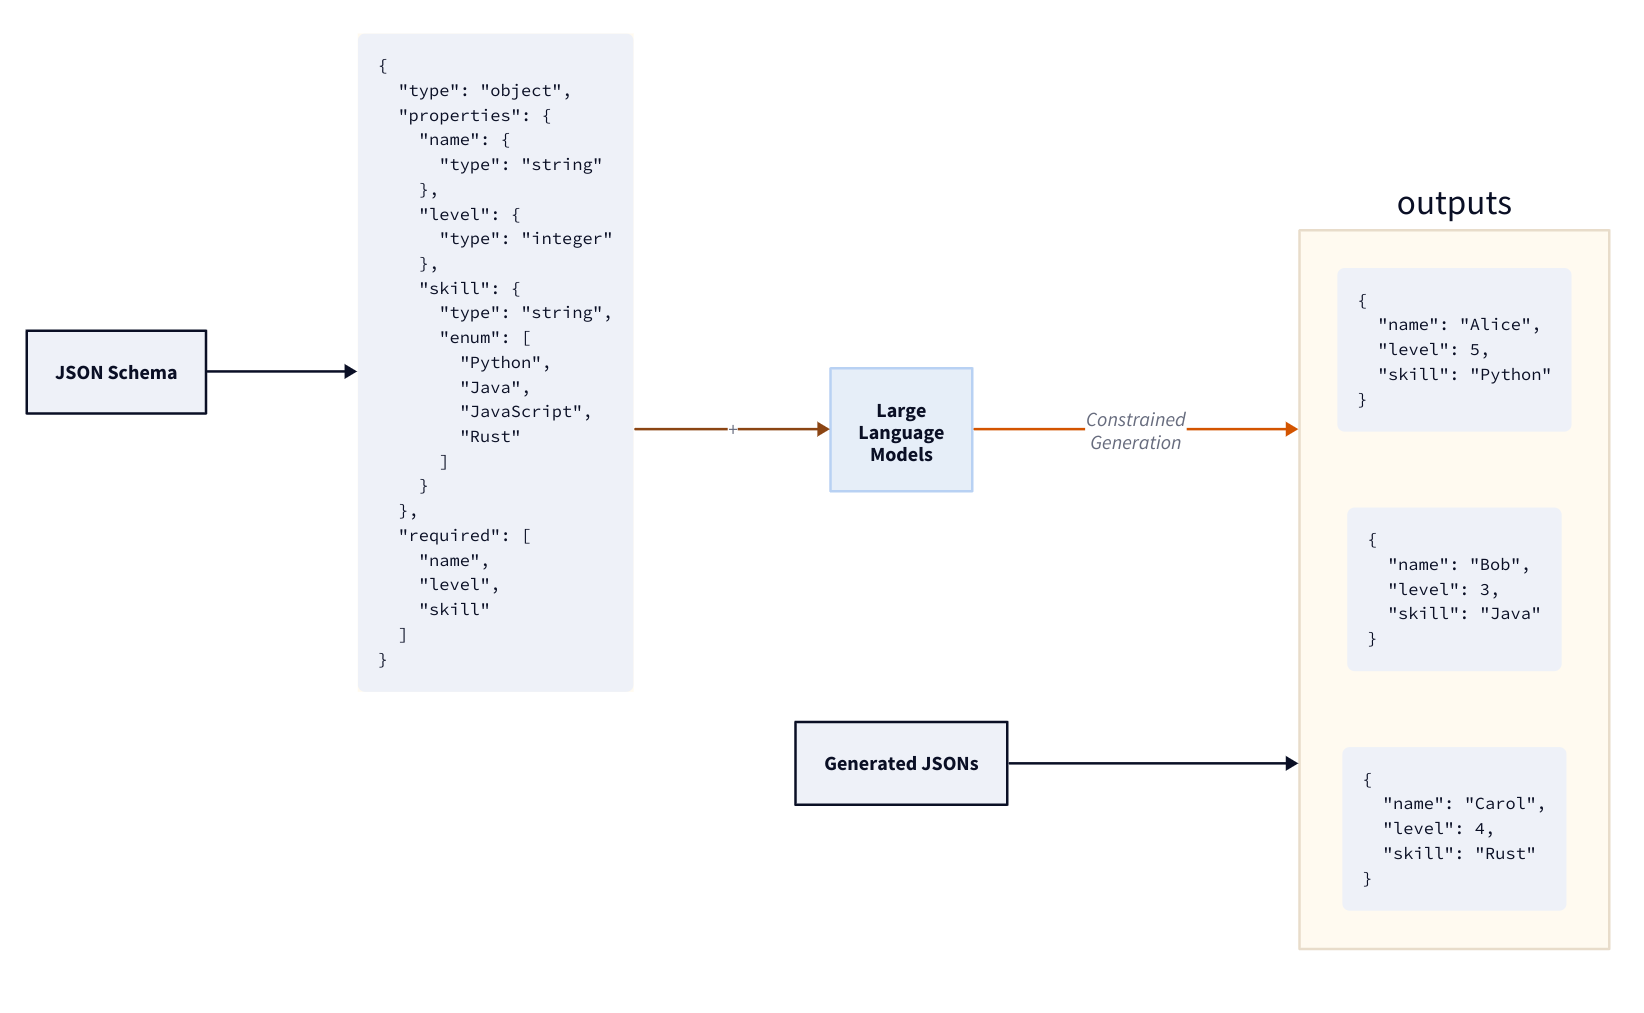
\includegraphics[scale=0.5]{structured_output/json.png}
\caption{Conceptual overview of JSON mode.}
\label{fig:json-mode}
\end{figure*}
When using JSON mode with OpenAI's API, it is recommended to instruct the model to produce JSON via some message in the conversation, for example via your system message. If you don't include an explicit instruction to generate JSON, the model may generate an unending stream of whitespace and the request may run continually until it reaches the token limit. To help ensure you don't forget, the API will throw an error if the string "JSON" does not appear somewhere in the context.

\begin{minted}{python}
prompt = f"""
Generate a two-person discussion about the key financial data from the following text in JSON format.
TEXT: {sec_filing}
"""
response = client.chat.completions.create(
    model="gpt-3.5-turbo",
    messages=[{"role": "user", "content": prompt}],
response_format = { "type": "json_object" }
)
\end{minted}

\begin{minted}{python}
response_content = response.choices[0].message.content
print(response_content)
\end{minted}
    \begin{verbatim}
    {
      "person1": "I see that Apple Inc. reported a total market value of approximately $2,628,553,000,000 held by non-affiliates as of March 29, 2024. That's a significant amount!",
      "person2": "Yes, it definitely shows the scale and value of the company in the market. It's impressive to see the sheer size of the market value.",
      "person1": "Also, they mentioned having 15,115,823,000 shares of common stock issued and outstanding as of October 18, 2024. That's a large number of shares circulating in the market.",
      "person2": "Absolutely, the number of shares outstanding plays a crucial role in determining the company's market capitalization and investor interest."
    }
    \end{verbatim}

This example solution is specific to OpenAI's API. Other LLM providers offer similar functionality, for example:

\begin{itemize}
    \item Google's Gemini offers JSON mode via response schema configuration.
    \item Anthropic \sidenote[][*10]{Isn't it surprising that Anthropic does not yet offer JSON and/or structured output generation to date? Isn't it even more surprising that today's recommended solution is to use function calling to get JSON responses even if you are not using the actual function in your application?} suggests tools use to get Claude to produce \href{https://docs.anthropic.com/en/docs/build-with-claude/tool-use#json-mode}{JSON output} that follows a schema.
\end{itemize}
\begin{marginlisting}[-1.35cm]
	\caption{Gemini's Structured Output.}
    \label{lst:gemini-structured}
	\vspace{0.6cm}
	\begin{lstlisting}[language=Python,style=kaolstplain]
llm_config = genai.generation_config={"response_mime_type": "application/json",
                   "response_schema": list[Round]}
	\end{lstlisting}
\end{marginlisting}


JSON mode is typically a form of fine-tuning, where a base model went though a post-training process to learn target formats. However, while useful this strategy is not guaranteed to work all the time.

\paragraph{A Note on "Guaranteed" Structured Output Mode}

In addition to JSON mode, it is worth mentioning that ``Structured Output''\index{Structured output} mode is also becoming popular among LLM providers. This is a feature that ensures the model will \textit{always} generate responses that adhere to your supplied JSON Schema.

Some benefits of Structured Outputs include:
\begin{itemize}
    \item \textbf{Reliable type-safety}: No need to validate or retry incorrectly formatted responses.
    \item \textbf{Explicit refusals}: Safety-based model refusals are now programmatically detectable.
    \item \textbf{Simpler prompting}: No need for strongly worded prompts to achieve consistent formatting.
\end{itemize}

Here's a Python example demonstrating how to use the OpenAI API to generate a structured output. We aim at extracting structured data from our sample SEC filing, in particular: (i) entities and (ii) places mentioned in the input doc. This example uses the \texttt{response\_format} parameter within the OpenAI API call. This functionality is supported by GPT-4o models, specifically \texttt{gpt-4o-mini}, \texttt{gpt-4o}, and later versions.

\begin{minted}[highlightlines={22}]{python}
from pydantic import BaseModel
from openai import OpenAI

class SECExtraction(BaseModel):
    mentioned_entities: list[str]
    mentioned_places: list[str]

def extract_from_sec_filing(sec_filing_text: str, prompt: str) -> SECExtraction:
    """
    Extracts structured data from an input SEC filing text.
    """
    client = OpenAI()
    completion = client.beta.chat.completions.parse(
        model="gpt-4o-mini",
        messages=[
            {
                "role": "system",
                "content": prompt
            },
            {"role": "user", "content": sec_filing_text}
        ],
        response_format=SECExtraction
    )
    return completion.choices[0].message.parsed
\end{minted}
\textbf{Explanation:}

\begin{itemize}
    \item \textbf{Data Structures:} The code defines one Pydantic model, \texttt{SECExtraction}, to represent the structured output of our parser. This model provides type hints and structure for the response.
    \item \textbf{API Interaction:} The \texttt{extract\_from\_sec\_filing} function uses the OpenAI client to send a chat completion request to the \texttt{gpt-4o-mini} model. The prompt instructs \sidenote[][*5]{Try omitting from the prompt one of the variables you want to extract (e.g. "places" or "entities"). You may find your API call fails to extract your target variables even with a proper pydantic model specified. That's how sensitive prompt engineering is when it comes to structured output generation. That's why we need an alternative approach which is the focus of the next section.} the model to extract our target attributes from input text. The \texttt{response\_format} is set to \texttt{SECExtraction}, ensuring the response conforms to the specified Pydantic model.
    \item \textbf{Output Processing:} The returned response is parsed into the \texttt{SECExtraction} model. The code then returns the parsed data.
\end{itemize}

\begin{minted}{python}
prompt_extraction = "You are an expert at structured data extraction. You will be given unstructured text from a SEC filing and extracted names of mentioned entities and places and should convert the response into the given structure."
sec_extraction = extract_from_sec_filing(sec_filing, prompt_extraction)
\end{minted}


\begin{minted}{python}
print("Extracted entities:", sec_extraction.mentioned_entities)
print("Extracted places:", sec_extraction.mentioned_places)
\end{minted}

\begin{verbatim}
    Extracted entities: ['Apple Inc.', 'The Nasdaq Stock Market LLC']
    Extracted places: ['Washington, D.C.', 'California', 'Cupertino, California']
\end{verbatim}


We observe that the model was able to extract the entities and places from the input text, and return them in the specified format.

The use of Pydantic models\index{Pydantic} and the \texttt{response\_format} parameter enforces the structure of the model's output, making it more reliable and easier to process.

This structured approach improves the reliability and usability of your application by ensuring consistent, predictable output from the OpenAI API.
This example solution is specific to OpenAI's API. That begs the question: How can we solve this problem generally for widely available open source LLMs? Enters logit post-processing.

\subsection{Logit Post-Processing}

Logit post-processing\index{Logit post-processing} is a technique that involves modifying the logits of the LLM's output before it is converted into text such that we have a ``controlled'' text generation.

The text generation process follows a probabilistic approach. At each step, the model calculates the probability distribution over its entire vocabulary to determine the most likely next token. 

Let's examine how an LLM processes an example prompt ``Is Enzo a good name for a baby?'' as depicted in Figure~\ref{fig:logit}:

\begin{enumerate}
    \item The tokenizer first segments the input text into tokens
    \item Each token gets mapped to a unique numerical ID
    \item The language model processes these token IDs through its deep neural network
    \item The model produces logits - unnormalized scores for each possible next token
    \item A softmax \sidenote{From raw logits to softmax probabilities:
$$P(y_i | x) = \text{softmax}(x_i) = \frac{e^{x_i}}{\sum_{j=1}^{n} e^{x_j}}
$$ for $i = 1,\ldots,n$ where, $P(y_i | x)$ represents the probability of class $i$ given input $x$ and $x_i$ is the logit (raw score) for class $i$.
} transformation converts these raw logits into a probability distribution
    \item The highest probability (3.25\%) indicates the model's strongest prediction for the next token
    \item Text generation then selects the next token based on a given strategy (e.g. greedy, top-k, etc)
\end{enumerate}



\begin{figure}[h]
\centering
\includesvg{structured_output/logit.svg}
    \caption{Text Generation Process.}
    \label{fig:logit}
\end{figure}

We can leverage the \texttt{transformers} library to extract the logits of the last token of the prompt.



\begin{minted}{python}
MODEL_NAME = "HuggingFaceTB/SmolLM2-1.7B-Instruct"
PROMPT = "Is Enzo a good name for a baby?"

from transformers import AutoTokenizer, AutoModelForCausalLM
import torch

tokenizer = AutoTokenizer.from_pretrained(MODEL_NAME)
model = AutoModelForCausalLM.from_pretrained(MODEL_NAME, 
    torch_dtype=torch.bfloat16, device_map="auto")
\end{minted}

After instantiating a small open source model \texttt{SmolLM2-1.7B-Instruct}, we can extract the logits of the last token given our prompt example "Is Enzo a good name for a baby?". We observe that the token 'I' ranks first with 3.25\% followed by ' What' with 3.05\%.

\begin{minted}{python}
inputs = tokenizer(PROMPT, return_tensors="pt").to(model.device)

# Get logits
with torch.inference_mode():
    outputs = model(**inputs)
    logits = outputs.logits

# Logits for the last token
last_token_logits = logits[:, -1, :]

next_token_probs = torch.nn.functional.softmax(last_token_logits, dim=-1)

k = 10
top_k_probs, top_k_indices = torch.topk(next_token_probs, k, dim=-1)

# Print the actual tokens, skipping special tokens
top_k_tokens = [tokenizer.decode(idx, skip_special_tokens=True) 
                for idx in top_k_indices[0]]

print(f"Top predicted tokens and probabilities:")
for prob, token in zip(top_k_probs[0][:k], top_k_tokens[:k]):
    if token.strip():  # Only print non-empty tokens
        print(f"'{token}': {prob:.4f}")
\end{minted}

\begin{verbatim}
Top predicted tokens and probabilities:
' I': 0.0325
' What': 0.0305
' Here': 0.0197
' Is': 0.0106
' My': 0.0093
\end{verbatim}


The main idea here is that we can modify the logits of the last token to bias the model towards the tokens we want to see in the output hence ``controlling'' the generation process.

The \texttt{transformers} library provides a \texttt{LogitsProcessor} class (see Listing \ref{lst:logit}) that allows us to modify the logits of the last token.

Without any logit processing, the model will generate the most likely token based on the probabilities.
\begin{minted}{python}
model.generate(**input)
\end{minted}
\begin{marginlisting}[-1.35cm]
	\caption{LogitsProcessor Class.}
    \label{lst:logit}
	\vspace{0.6cm}
	\begin{lstlisting}[language=Python,style=kaolstplain]
class LogitsProcessor:
    """Abstract base class for all logit processors that can be applied during generation."""

    def __call__(self, input_ids: torch.LongTensor, scores: torch.FloatTensor) -> torch.FloatTensor:
	\end{lstlisting}
\end{marginlisting}
With logit processing, we can modify the logits of the last token to bias the model towards the tokens we want to see in the output.
\begin{minted}{python}
model.generate(**input, logits_processor=LogitsProcessorList([CustomLogitsProcessor()]))
\end{minted}

Here, \texttt{CustomLogitsProcessor} is an example of a user-defined custom logits processor concrete class we would pass to \texttt{model.generate()} to instruct our goal to control the generation process. This class should implement the abstract \texttt{LogitsProcessor} class from the \texttt{transformers}\index{Transformers} library.

The \texttt{LogitsProcessor} provides a unified interface for modifying prediction scores during text generation with language models. It acts as an intermediary step between the raw logits output by the model and the final token selection process:

\begin{enumerate}
    \item Input: Takes sequence tokens (input\_ids) and prediction scores (scores tensor)
    \item Output: Returns modified scores that influence the next token selection
\end{enumerate}

Importantly, it defines the \texttt{\_\_call\_\_} method that takes two key arguments:

\begin{enumerate}
    \item input\_ids (torch.LongTensor): 
    \begin{itemize}
        \item Shape: (batch\_size, sequence\_length)
        \item Contains the token IDs of the input sequence
        \item Obtained through tokenizer.encode() or tokenizer.\_\_call\_\_()
    \end{itemize}
    
    \item scores (torch.FloatTensor):
    \begin{itemize}
        \item Shape: (batch\_size, vocab\_size) 
        \item Raw logits from the language model head
        \item Can be pre-softmax or post-softmax scores
        \item Represents prediction probabilities for each token
    \end{itemize}
\end{enumerate}

The method returns:
\begin{itemize}
    \item torch.FloatTensor with shape (batch\_size, vocab\_size)
    \item Contains the modified prediction scores after processing
\end{itemize}

This allows for custom manipulation of the scores before token selection, enabling fine-grained control over the generation process.

Let's go through a concrete example to better understand how we can control output generation.

Let's suppose we want to bias the model towards the tokens ``Yes'' and ``No'' in the output. That is, we would like the model to always return ``Yes'' or ``No'' in the output to our prompt (in this example ``Is Enzo a good name for a baby?''). 

A naive approach would be to modify the logits of the last token by masking out all tokens except ``Yes'' and ``No''. We can then pick the most likely token (from ``Yes'' or ``No'') as the output in a greedy fashion.

The \texttt{YesNoLogitsProcessor} class below implements this naive greedy approach by implementing a custom \texttt{LogitsProcessor}~\sidenote{In this stylized logits processor example, we simply mask all token bar "Yes" and "No" and then calculate their logits post-making returning the most likely token as response. We will discuss in the next sections how to generalize this simple idea using grammers and finite-state machines.}.

\begin{minted}{python}
class YesNoLogitsProcessor(LogitsProcessor):
    def __init__(self, yes, no, tokenizer, initial_length):
        self.yes = yes
        self.no = no
        self.tokenizer = tokenizer
        self.initial_length = initial_length
        
    def __call__(self, input_ids: torch.LongTensor, scores: torch.FloatTensor) -> torch.FloatTensor:
        # If we already generated a response, mask everything
        if len(input_ids[0]) > self.initial_length:
            scores.fill_(-float('inf'))
            return scores
            
        # Debug prints
        yes_tokens = self.tokenizer.encode(self.yes, add_special_tokens=False)
        no_tokens = self.tokenizer.encode(self.no, add_special_tokens=False)
        print(f"Yes token ID: {yes_tokens}")
        print(f"No token ID: {no_tokens}")
        
        
        # Extract original logits for yes/no
        yes_no_logits = scores[:, [yes_tokens[0], no_tokens[0]]]
        print(f"[Yes, No] logits: {yes_no_logits}")
        
        # Get probabilities using softmax
        yes_no_probs = torch.nn.functional.softmax(yes_no_logits, dim=-1)
        yes_prob = yes_no_probs[:, 0]
        no_prob = yes_no_probs[:, 1]
        print(f"Yes prob: {yes_prob}")
        print(f"No prob: {no_prob}")
        
        # Mask all tokens with -inf
        scores.fill_(-float('inf'))
        
        # Set the higher probability choice to 0
        yes_mask = yes_prob > no_prob
        scores[:, yes_tokens[0]] = torch.where(yes_mask, torch.tensor(1e4), torch.tensor(-float('inf')))
        scores[:, no_tokens[0]] = torch.where(~yes_mask, torch.tensor(1e4), torch.tensor(-float('inf')))
        
        return scores
\end{minted}

We can simply pass our custom logits processor to \texttt{model.generate()} method to test our controlled generation.

\begin{minted}{python}
input_ids = tokenizer.encode(PROMPT, return_tensors="pt")
initial_length = len(input_ids[0])

YES = "yes"
NO = "no"

# Controlled generation
generation_output_controlled = model.generate(**inputs, logits_processor=LogitsProcessorList([YesNoLogitsProcessor(YES, NO, tokenizer, initial_length)]), max_length=50)

# Uncontrolled generation
generation_output = model.generate(**inputs, max_length=50)
\end{minted}

Below we print the ``Yes'' and ``No'' token IDs, the logits of the last token (raw scores before masking) and then the probabilities of the tokens ``Yes'' and ``No'' after masking and softmax normalization. In this run, the model predicts ``Yes'' with a probability of 0.4263 and ``No'' with a probability of 0.5737, post-masking. In our greedy approach, our custom logits processor will pick the most likely token, in this case ``No''.

\begin{verbatim}
Yes token ID: [10407]
No token ID: [4607]
[Yes, No] logits: tensor([[2.6250, 2.9219]])
Yes prob: tensor([0.4263])
No prob: tensor([0.5737])
\end{verbatim}

Let's see if it works as expected. We write a helper function to extract the response from the model's generation output.

\begin{minted}{python}
def generate_response(model_output, tokenizer):
    gen_output = tokenizer.batch_decode(model_output, skip_special_tokens=True, clean_up_tokenization_spaces=False)
    generated_text = gen_output[0][
                len(
                    tokenizer.decode(
                        inputs["input_ids"][0], skip_special_tokens=True
                    )
                ) :
            ].strip()
    return generated_text
\end{minted}

Controlled generation using our custom logits processor:

\begin{minted}{python}
generate_response(generation_output_controlled, tokenizer)
\end{minted}

\begin{verbatim}
'no'
\end{verbatim}

Regular generation \sidenote{We limit text generation to 50 tokens output.}:

\begin{minted}{python}
generate_response(generation_output, tokenizer)
\end{minted}

\begin{verbatim}
'Enzo is a classic Italian name that'
\end{verbatim}

As we can see, our controlled generation returned ``No'' to our prompt while the regular generation returned a more verbose response, as expected.

Here, we provided a simple greedy approach to logit post-processing using transformers library in a process that can be extended and customized to more complex logit post-processing tasks \sidenote{A more robust approach would define a grammar to control output generation as we will demonstrate in the next section.}. There are some higher level libraries that can help us streamline this process while offering some flexibility and control such as Outlines. We will cover this library as well as other tools such as Ollama and Langchain in the following sections each one offering a different approach to structured output with varying degrees of control and flexibility.

\section{Tools}

\subsection{Outlines}

Outlines\index{Outlines} \sidecite{outlines2024} is a library specifically focused on structured text generation from LLMs. Under the hood, Outlines works by adjusting the probability distribution of the model's output logits - the raw scores from the final layer of the neural network that are normally converted into text tokens. By introducing carefully crafted logit biases, Outlines can guide the model to prefer certain tokens over others, effectively constraining its outputs to a predefined set of valid options.

The authors solve the general guided generation problem \sidecite{willard2023efficientguidedgenerationlarge}, which, as a consequence, solves the problem of structured output generation in LLMs by introducing an efficient indexing approach that reformulates neural text generation using finite-state machines (FSMs) \sidenote{A Finite State Machine (FSM) is a computational model that consists of a finite number of states and transitions between those states, where the system can be in only one state at a time and moves between states based on inputs or conditions.}.

They define the next token generation as a random variable:

\[s_{t+1} \sim \text{Categorical}(\alpha) \text{ where } \alpha = \text{LLM}(S_t, \theta)\]

Where:

\begin{itemize}
    \item $s_{t+1}$ is the next token to be generated
    \item $S_t = (s_1...s_t)$ represents a sequence of t tokens with $s_t \in V$
    \item $V$ is the vocabulary with size $|V| = N$ (typically around $10^4$ or larger)
    \item $\alpha \in \mathbb{R}^N$ is the output logits/probabilities over the vocabulary
    \item $\theta$ is the set of trained parameters of the LLM
    \item $\text{LLM}$ refers to a deep neural network trained on next-token-completion tasks
    \item $\text{Categorical}(\alpha)$ represents sampling from a categorical distribution with probabilities $\alpha$
\end{itemize}

When applying masking for guided generation, this becomes:

\[\tilde{\alpha} = m(S_t) \odot \alpha\]

\[\tilde{s}_{t+1} \sim \text{Categorical}(\tilde{\alpha})\]

Where:

\begin{itemize}
    \item $m: P(V) \rightarrow {0,1}^N$ is a boolean mask function
    \item $\odot$ represents element-wise multiplication
    \item $\tilde{\alpha}$ is the masked (constrained) probability distribution
    \item $\tilde{s}_{t+1}$ is the next token sampled under constraints
\end{itemize}
This formulation allows the masking operation to guide the generation process by zeroing out probabilities of invalid tokens according to the finite state machine states. But instead of checking the entire vocabulary (size $N$) at each generation step ($O(N)$ complexity)\sidenote{$O(N)$ complexity simply means that the algorithm's execution time grows linearly the size of the vocabulary.} to enforce output constraints, they convert constraints (regex/grammar) into FSM states and build an index mapping FSM states to valid vocabulary tokens. This achieves $O(1)$ average complexity for token generation.

In summary, there are two stages in the Outlines framework \sidecite{vivien2024regex}:

\begin{enumerate}
    \item \textbf{Preprocessing Step}: Outlines converts a character-level deterministic finite automaton (DFA) testing whether a string matches a regex into a token-level DFA testing whether a token sequence is decoded in a string matching the regex.

    \item \textbf{Decoding Step}: At decoding time, the DFA is used to determine, for each new token, which potential tokens are allowed. Starting from the initial state of the DFA, the allowed tokens are determined by the outgoing transitions from the current state. The corresponding mask is applied to the next token probabilities and these probabilities are renormalized. A new token can then be sampled and the state of the DFA updated.
\end{enumerate}

\begin{marginfigure}
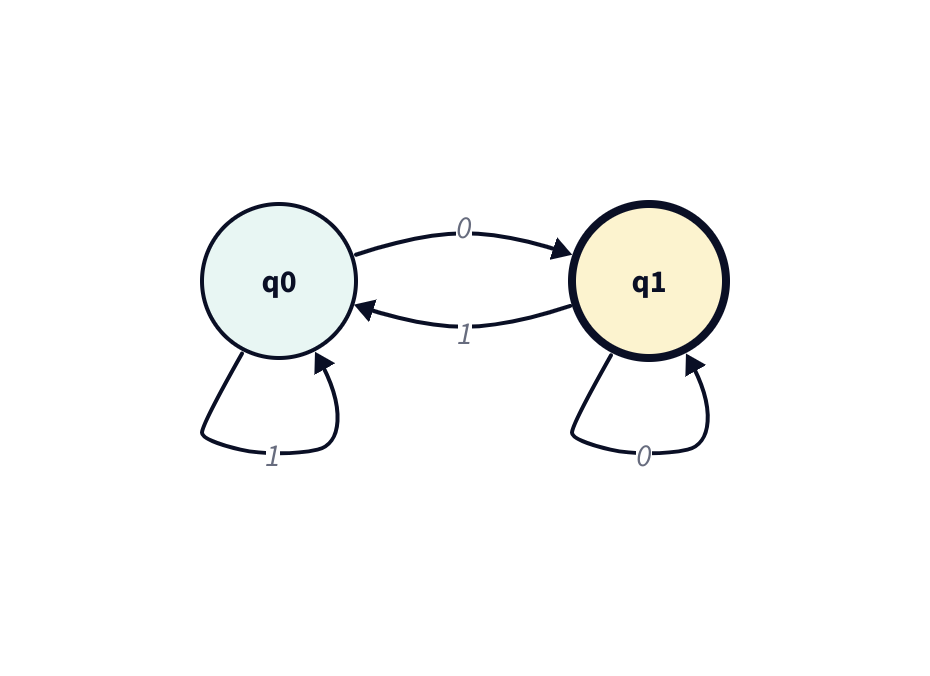
\includegraphics{structured_output/dfa.png}
\caption[DFA Example]{A DFA is a computational model that processes input one symbol at a time, moving between a finite set of states in a deterministic way. Hence, DFA is a subset of FSM with additional constraints that make it deterministic.}
\end{marginfigure}

At each step, the model's probability distribution is masked and renormalized according to the current state and valid transitions.

As an example, let's suppose we want to constrain the output of an LLM to the following set of options: 
\begin{itemize}
    \item Y/yes
    \item N/no  
    \item N/never
    \item A/always
\end{itemize}

This can be done by creating a state machine that has a start state, an end state and a set of valid transitions between states with possible states represented as the following regex string: 

\begin{minted}{python}
r"\textbackslash s*([Yy]es|[Nn]o|[Nn]ever|[Aa]lways)"
\end{minted}

The state machine in Fig.~\ref{fig:outlines-state-machine} illustrates how Outlines works under the hood, where:
\begin{itemize}
    \item Prop: Represents the logit token probability given by the LLM
    \item Mask: Mask value of the transition as defined by the state machine  
    \item Final: The renormalized token probability post-masking
\end{itemize}

\begin{figure*}[htbp]
\centering
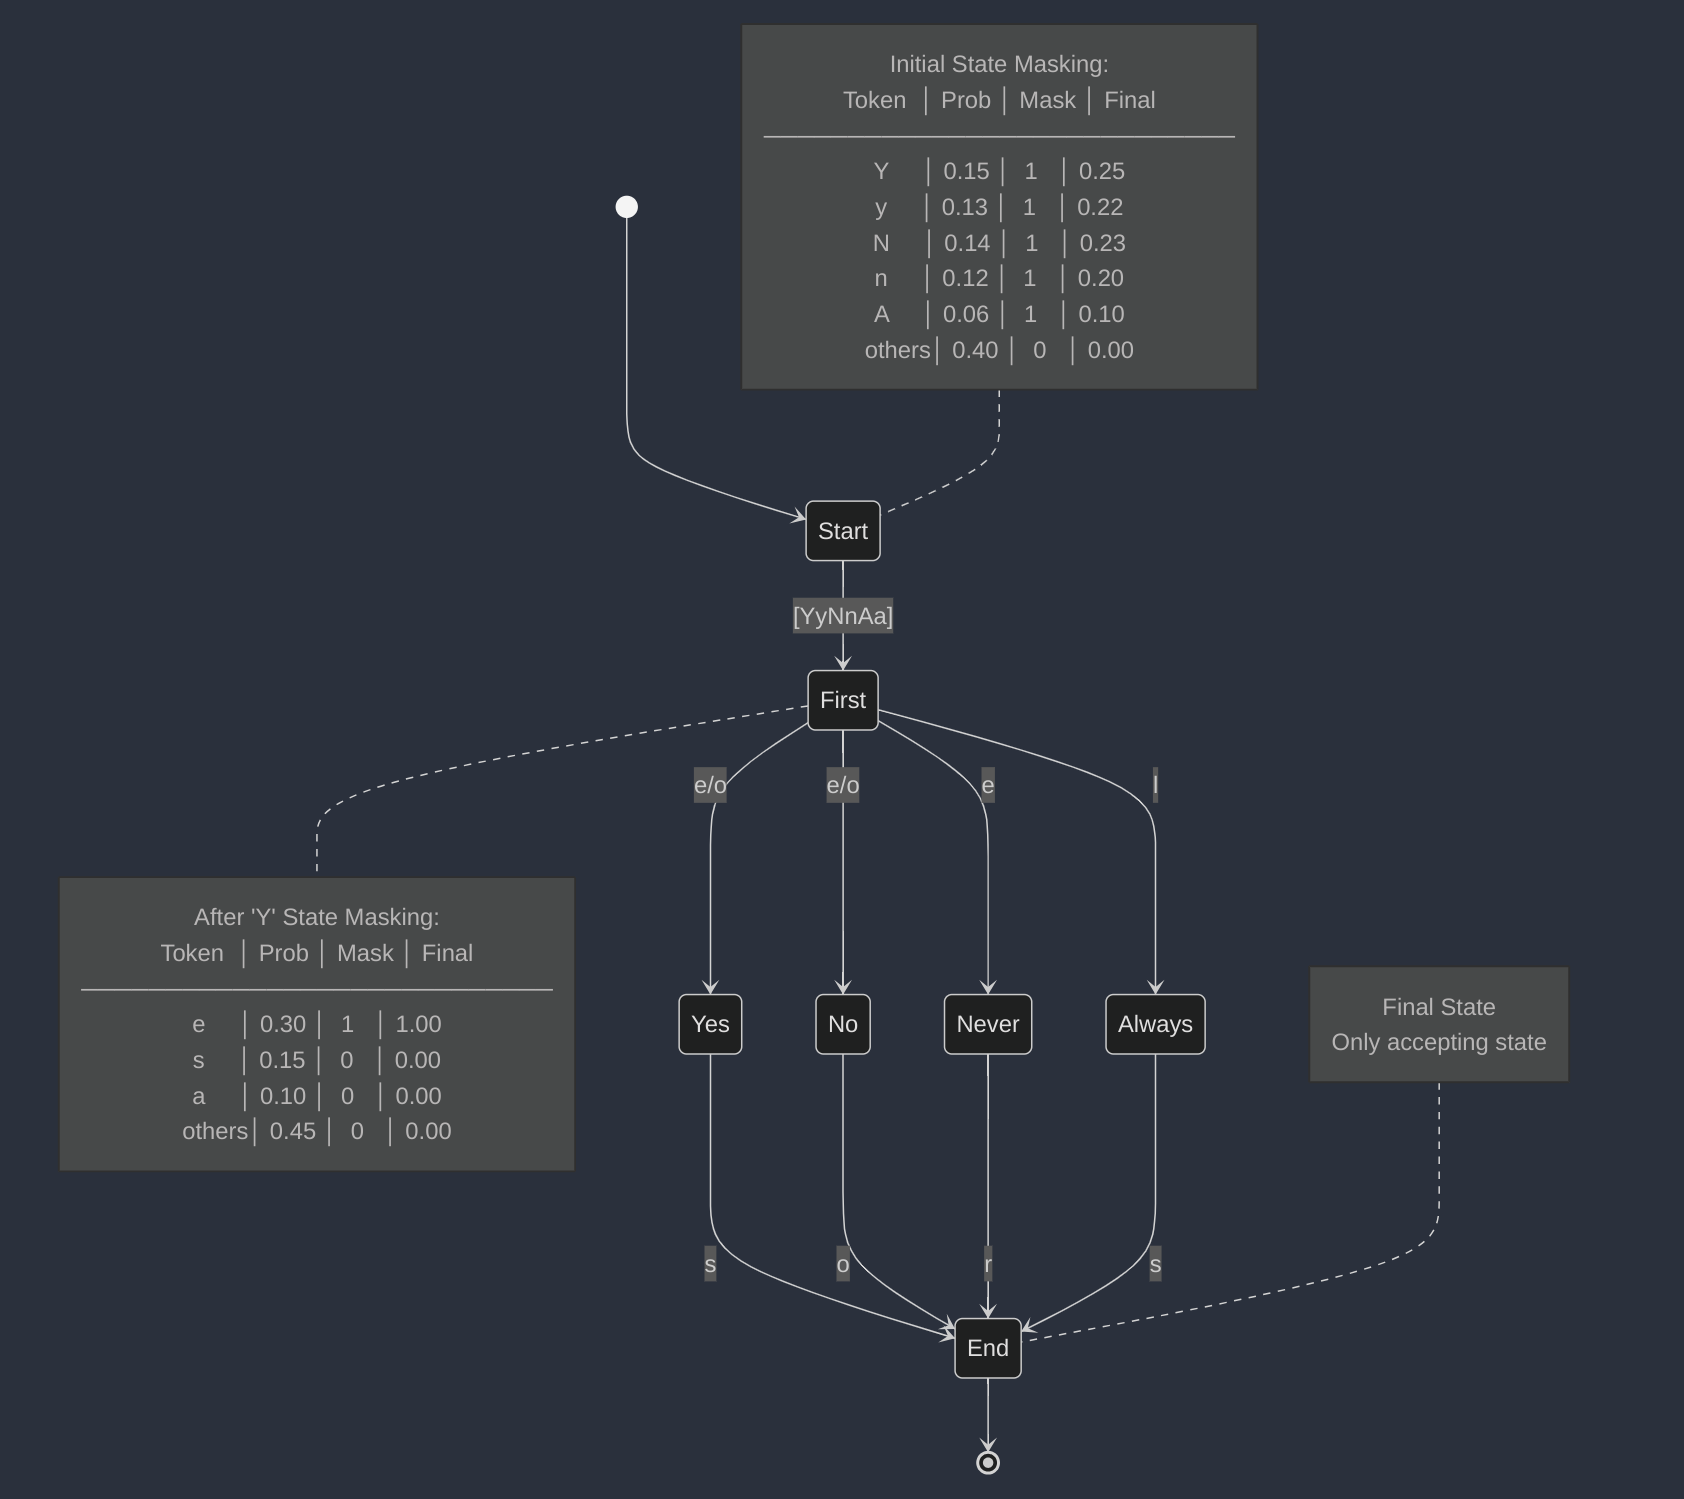
\includegraphics[width=1.4\textwidth]{structured_output/outlines_state_machine.png}
\caption{Outlines State Machine \cite{vivien2024regex}}
\label{fig:outlines-state-machine}
\end{figure*}

The initial ``Start'' state contains a masking table that controls which tokens can begin the sequence. In this example, only characters from the set \texttt{[YyNnAa]} are allowed as valid first characters, with each having an assigned probability and mask value. The masking mechanism effectively filters out invalid tokens by setting their mask values to 0, ensuring only permitted transitions to the ``First'' state.

After transitioning to the ``First'' state, the system continues to use probability masking to guide the sequence. For example, when receiving `Y' as input, the masking table adjusts token probabilities to ensure valid continuations.

This finite state machine architecture serves multiple purposes in controlling text generation:

\begin{enumerate}
    \item Managing token probabilities through strategic masking
    \item Preventing invalid token sequences 
    \item Enforcing specific token patterns
    \item Providing fine-grained control over token generation and validation
\end{enumerate}

In that way, Outlines, the Python package, provides several powerful controlled generation features for developers:
\begin{itemize}
    \item \textbf{Regex-based structured generation}: Guide the generation process using regular expressions.
    \item \textbf{Multiple Choice Generation}: Restrict the LLM output to a predefined set of options.
    \item \textbf{Pydantic model}: Ensure the LLM output follows a Pydantic model.
    \item \textbf{JSON Schema}: Ensure the LLM output follows a JSON Schema.
\end{itemize}

Outlines can support major proprietary LLM APIs (e.g. OpenAI via vLLM). However, one of its key advantages is the ability to ensure structured output for Open Source models, which often lack such guarantees by default.

\begin{minted}{bash}
pip install outlines
pip install transformers
\end{minted}

In this example, we will use a \texttt{Qwen2.5-0.5B}\index{Qwen} model \sidenote{Chapter \ref{chapter:local} presents some remarkable performance data on Qwen2.5 models, which are one of them best Open Source models available today}, a lightweight open source model from Alibaba Cloud known for its strong performance despite its small size.

\begin{minted}{python}
import outlines

model = outlines.models.transformers("Qwen/Qwen2.5-0.5B-Instruct")
\end{minted}

\begin{minted}{python}
TOP = 100
prompt = f"""You are a sentiment-labelling assistant specialized in Financial Statements.
Is the following document positive or negative?

Document: {sec_filing[:TOP]}
"""

generator = outlines.generate.choice(model, ["Positive", "Negative"])
answer = generator(prompt)
print(answer)
\end{minted}

\begin{verbatim}
    Negative
\end{verbatim}

In this simple example, we use Outlines' \texttt{choice} method to constrain the model output to a predefined set of options (``Positive'' or ``Negative''). This ensures the model can only return one of these values, avoiding any unexpected or malformed responses.

Outlines also allows to guide the generation process so the output is guaranteed to follow a JSON schema or a Pydantic model. We will go back to our example of extracting entities and places from a SEC filing. In order to do so, we simply need to pass our Pydantic model to the \texttt{json} method in Outlines' \texttt{generate} module.

\begin{minted}{python}
BASE_PROMPT = "You are an expert at structured data extraction. You will be given unstructured text from a SEC filing and extracted names of mentioned entities and places and should convert the response into the given structure."
\end{minted}

\begin{minted}{python}
prompt = f"{BASE_PROMPT} Document: {sec_filing[:TOP]}"
generator = outlines.generate.json(model, SECExtraction)
sec_extraction_outlines = generator(prompt)
\end{minted}

\begin{minted}{python}
print("Extracted entities:", sec_extraction_outlines.mentioned_entities)
print("Extracted places:", sec_extraction_outlines.mentioned_places)
\end{minted}

\begin{verbatim}
    Extracted entities: ['Zsp', 'ZiCorp']
    Extracted places: ['California']
\end{verbatim}

We observe that the model was able to extract the entities and places from the input text, and return them in the specified format. However, it is interesting to see that the model hallucinates a few entities, a phenomenon that is common for smaller Open Source models that were not fine-tuned on the task of entity extraction \sidenote{An alternative approach would be to define a valid set of entities to be extracted in order to avoid hallucination.}.
\subsection{LangChain}

LangChain\index{LangChain} \cite{langchain_github} is a framework designed to simplify the development of LLM applications. It provides an abstraction layer over many LLM providers that in turn offers structured output.

In particular, LangChain offers the \texttt{with\_structured\_output} method, which can be used with LLMs that support structured output APIs, allowing you to enforce a schema directly within the prompt.

\begin{quote}
\texttt{with\_structured\_output} takes a schema as input which specifies the names, types, and descriptions of the desired output attributes. The method returns a model-like Runnable, except that instead of outputting strings or messages it outputs objects corresponding to the given schema. The schema can be specified as a TypedDict class, JSON Schema or a Pydantic class. If TypedDict or JSON Schema are used then a dictionary will be returned by the Runnable, and if a Pydantic class is used then a Pydantic object will be returned.
\end{quote}

\begin{minted}{bash}
pip install -qU langchain-openai
\end{minted}

\begin{minted}[highlightlines={10}]{python}
from langchain_openai import ChatOpenAI
from langchain_core.prompts import ChatPromptTemplate
def extract_from_sec_filing_langchain(sec_filing_text: str, 
    prompt: str) -> SECExtraction:
    """
    Extracts structured data from an input SEC filing text using LangChain.
    """
    llm = ChatOpenAI(model="gpt-4o-mini")

    structured_llm = llm.with_structured_output(SECExtraction)

    prompt_template = ChatPromptTemplate.from_messages(
        [
            ("system", prompt),
            ("human", "{sec_filing_text}"),
        ]
    )

    llm_chain = prompt_template | structured_llm
    
    return llm_chain.invoke(sec_filing_text)
\end{minted}


\begin{minted}{python}
prompt_extraction = """You are an expert at structured data extraction. 
You will be given unstructured text from a SEC filing and 
extracted names of mentioned entities and places and should convert the response into the given structure."""
sec_extraction_langchain = extract_from_sec_filing_langchain(
    sec_filing, prompt_extraction)
\end{minted}

\begin{minted}{python}
print("Extracted entities:", sec_extraction_langchain.mentioned_entities)
print("Extracted places:", sec_extraction_langchain.mentioned_places)
\end{minted}

\begin{verbatim}
Extracted entities: ['Apple Inc.']
Extracted places: ['California', 'Cupertino']
\end{verbatim}

We observe that the model was able to extract the entities and places from the input text, and return them in the specified format. A full list of models that support \texttt{.with\_structured\_output()} can be found \href{https://python.langchain.com/docs/integrations/chat/#featured-providers}{here}. You can also use Outlines with LangChain \sidecite{langchain2024outlines}.
\subsection{Ollama}

Ollama\index{Ollama} \cite{ollama2024website} is a popular tool that allows you to run LLMs locally (see \label{chapter:local} for additional details). Ollama first introduced structured output generation in version 0.5.1 in late 2024 providing support for JSON output but highlighting additional formats are coming soon.

The current \texttt{ollama} implementation leverages LLama.cpp\index{LLama.cpp} GBNF (GGML BNF) grammars \sidecite{llama_cpp_grammars} to enable structured output generation. LLama.cpp GBNF forces language models to generate output in specific, predefined formats by constraining their outputs to follow precise rules and patterns. The system accomplishes this through a formal grammar specification that defines exactly how valid outputs can be constructed. It's essentially an extension of BNF (Backus-Naur Form) \sidecite{backus_naur_form} with some modern regex-like features added. These rules carefully define what elements are allowed, how they can be combined, and what patterns of repetition and sequencing are valid. By enforcing these constraints during generation, GBNF ensures the model's output strictly adheres to the desired format.\sidenote{As a simple BNF example, this grammar defines basic arithmetic expressions with numbers, addition, subtraction, and parentheses.
\[
\begin{aligned}
\langle \text{expr} \rangle &::= \langle \text{number} \rangle \\
    &\mid \langle \text{expr} \rangle \text{ `}+\text{' } \langle \text{expr} \rangle \\
    &\mid \langle \text{expr} \rangle \text{ `-' } \langle \text{expr} \rangle \\
    &\mid \text{`(' } \langle \text{expr} \rangle \text{ `)'} \\
\langle \text{number} \rangle &::= \langle \text{digit} \rangle \mid \langle \text{number} \rangle \langle \text{digit} \rangle \\
\langle \text{digit} \rangle &::= \text{`0'} \mid \text{`1'} \mid \text{`2'} \mid \text{`3'} \mid \text{`4'} \mid \text{`5'} \mid \text{`6'} \mid \text{`7'} \mid \text{`8'} \mid \text{`9'}
\end{aligned}
\]
}

Let's replicate our previous structured output generation example with Ollama. First, make sure you have Ollama installed. You can find installation instructions \href{https://ollama.com/docs/installation}{here}.

\begin{minted}{bash}
curl -fsSL https://ollama.com/install.sh | sh
pip install ollama
\end{minted}

The code below demonstrates how to use Ollama's structured output capabilities with a Pydantic model as we did before with OpenAI, LangChain and Outlines. 

The \texttt{SECExtraction} pydantic model defines the expected structure with two fields: mentioned\_entities and mentioned\_places as lists of strings we expect the model to return given an input SEC filing. The \texttt{extract\_entities\_from\_sec\_filing} function uses Ollama's chat API to analyze SEC filings and extract entities in a structured format, with temperature set to 0 for deterministic results. We pass the Pydantic model's JSON schema to Ollama via the \texttt{format} parameter. We append a suffix to the prompt instructing the model to return the response as JSON ("Return as JSON.") as recommended by Ollama maintainers.

\begin{minted}[highlightlines={8, 27, 33}]{python}
from ollama import chat
from pydantic import BaseModel

class SECExtraction(BaseModel):
    mentioned_entities: list[str]
    mentioned_places: list[str]

OLLAMA_STRUCTURED_OUTPUT_PROMPT_SUFFIX = "Return as JSON."
OLLAMA_STRUCTURED_OUTPUT_TEMPERATURE = 0

def extract_entities_from_sec_filing(doc: str, model: str) -> dict:
    """
    Extract entities and places from an SEC filing using Ollama chat.
    
    Args:
        doc: The SEC filing text to analyze
        model: The Ollama model to use for extraction
        
    Returns:
        The raw response from the chat model
    """
    response = chat(
        messages=[
            {
                'role': 'user',
                'content': f"""{BASE_PROMPT}
                {OLLAMA_STRUCTURED_OUTPUT_PROMPT_SUFFIX}
                
                Document: {doc}"""
            }
        ],
        model=model,  # You can also use other models like 'mistral' or 'llama2-uncensored'
        format=SECExtraction.model_json_schema(),
        options={'temperature': OLLAMA_STRUCTURED_OUTPUT_TEMPERATURE}  # Set to 0 for more deterministic output
    )
    return response
\end{minted}

We can now run the function and print the extracted entities and places. But first we need to start the Ollama server with our target LLM model (Qwen2.5-0.5B) running locally.

\begin{minted}{bash}
ollama run qwen2.5:0.5b
\end{minted}

\begin{minted}{python}
doc = sec_filing[:TOP]
model = "qwen2.5:0.5b"

response = extract_entities_from_sec_filing(doc, model)

import json
response_json = json.loads(response.message.content)
\end{minted}

\begin{minted}{python}
print("Extracted entities:", response_json.get('mentioned_entities'))
print("Extracted places:", response_json.get('mentioned_places'))
\end{minted}

\begin{verbatim}
Extracted entities: ['United States', 'SECURITIES AND EXCHANGE COMMISSION']
Extracted places: []
\end{verbatim}

The extracted entities and places were quite different from those previously extracted using Outlines and Langchain, as expected since this depends mostly on the underlying model which is quite small in this example. We do observe though that we have successfully obtained results in JSON format as specified.

\section{Discussion}

\subsection{Best Practices}

When implementing structured output with LLMs, it's crucial to understand the distinction between different approaches. Some methods, such as logit post-processing, provide mathematical guarantees that the output will conform to the specified structure. This contrasts sharply with approaches like JSON mode, which rely on fine-tuned models or prompt engineering that offer no formal guarantees. This distinction becomes particularly important in production environments where reliability and consistency are paramount. With that in mind, here are some best practices to consider when implementing structured output generation with LLMs:

\begin{itemize}
    \item \textbf{Clear Schema Definition}: Define the desired output structure clearly. This can be done in several ways including schemas, types, or Pydantic\index{Pydantic} models as appropriate.
    
    \item \textbf{Descriptive Naming}: Use meaningful names for fields and elements in your schema.
    
    \item \textbf{Integration}: If you are connecting the model to tools, functions, data, etc. in your system, then you are highly encouraged to use a typed structured output (e.g. Pydantic models) to ensure the model's output can be processed correctly by downstream systems.
\end{itemize}

\begin{kaobox}[frametitle=Important]
Order matters when generating an LLM response! Results performance can significantly vary depending on whether the LLM is asked to provide a score first and then explanation next versus the opposite way around. A "Think Before You Speak" strategy is recommended, i.e. to place score explanation first and the actual resulting score next can improve results~\sidecite{xie2024ordermattershallucinationreasoning, openai2024cookbookissue}.
\end{kaobox}

In summary, first one needs to clearly define the typed structure LLM applications will interface with, then determine whether strong guarantees are needed in order to determine tradeoffs between control and ease of implementation.

\subsection{Comparing Solutions}

The choice of framework for structured LLM output depends heavily on specific constraints, requirements and use cases. LangChain is the most used LLM framework today with a large developer community base however its structured output generation depends on the underlying LLM provider support. Ollama enables straightforward local deployment and experimentation democratizing access to LLMs while fostering privacy and control, however today it only offers JSON format with further formats to come. Outlines emerges as a solution that provides formal guarantees with great flexibility and control over structured output generation while providing support for a wide range of LLMs. Table~\ref{structured_output_frameworks} provides a summary comparison of the different solutions.

\begin{table*}[h]
\caption{Structured Output Frameworks Comparison}
\label{structured_output_frameworks}
\begin{tabular}{|p{0.15\textwidth}|p{0.25\textwidth}|p{0.3\textwidth}|p{0.3\textwidth}|}
\hline
\textbf{Feature} & \textbf{LangChain} & \textbf{Outlines} & \textbf{Ollama} \\
\hline
\textbf{Approach} & Wrapper around LLM's native structured output APIs using with\_structured\_output method & Adjusts probability distribution of model's output logits to guide generation & Uses llama.cpp GBNF grammars to constrain output format \\
\hline
\textbf{Model Support} & Limited to LLMs with built-in structured output APIs & Broad support for open-source models via transformers, llama.cpp, exllama2, mlx-lm and vllm & Broad support focused on enabling running open-source models locally \\
\hline
\textbf{Output Format Support} & - TypedDict\newline - JSON Schema\newline - Pydantic class & - Multiple choice generation\newline - Regex-based structure\newline - Pydantic model\newline - JSON Schema & - Currently JSON only\newline - Additional formats planned \\
\hline
\textbf{Key Advantages} & - Simple integration with supported LLMs & - Provides guarantees on output structure\newline - Fine-grained control over generation\newline - Strong open-source model support & - Excellent for local deployment\newline - Simple setup and usage\newline - Built-in model serving \\
\hline
\textbf{Use Case Focus} & Enterprise applications using commercial LLMs & Applications requiring output control guarantees or using open-source models & Local deployment and/or experimentation \\
\hline
\end{tabular}
\end{table*}

Other related tools not covered in this chapter worth mentioning include Guidance \cite{guidance2024repo}, Instructor \cite{instructorgithub}, LM Format Enforcer \cite{lmformatenforcergithub}, and NVIDIA's Logits Processor Zoo \cite{nvidia2024logitsprocessorzoo}.

\subsection{Research and Ongoing Debate}

The use of structured output for Large Language Models is a developing area. While the ability to constrain LLM outputs offer clear benefits in parsing, robustness, and integration, there is growing debate on whether it also potentially comes at the cost of performance as well as reasoning abilities. Research in this area should be taken with a grain of salt since findings are mixed and often depend on the specific task and model family at hand furthermore model families are not always comparable and are getting updated by the day! Nonetheless, early findings provide some interesting insights as to why there is no one-size-fits-all solution when it comes to LLMs structured output.

There is some evidence indicating that LLMs may have bias in their handling of different output formats \sidecite{long2024llms}. This study examined common output structures like multiple-choice answers, wrapped text, lists, and key-value mappings. The authors analyzed key LLM model families, namely Gemma\index{Gemma}, Mistral\index{Mistral}, and ChatGPT\index{ChatGPT}, uncovering bias across multiple tasks and formats. The researchers attributed these biases to the models' underlying token distributions for different formats. An example of this format bias emerged in the comparison between JSON and YAML outputs. While models like Mistral and Gemma excelled at generating JSON structures, they performed notably worse with YAML. Their YAML outputs often contained extraneous information that degrades output quality. This disparity likely stems from JSON's prevalence in training data, highlighting how a format's popularity directly influences model performance. While the studied models can be probably considered outdated by now since models are getting updated on a rapidly fashion, it is important to remark that addressing format bias is critical for advancing LLMs and ensuring their reliable application in real-world scenarios.

Recent (not yet peer-reviewed) research ``Let Me Speak Freely? A Study on the Impact of Format Restrictions on Performance of Large Language Models'' \sidecite{tam2024letspeakfreelystudy} suggests that imposing format restrictions on LLMs might impact their performance, particularly in reasoning-intensive tasks. Further evidence \sidecite{aider2024codejson} suggests LLMs may produce lower quality code if they're asked to return it as part of a structured JSON response, in particular:

\begin{itemize}
    \item \textbf{Potential performance degradation:} Enforcing structured output, especially through constrained decoding methods like JSON-mode, can negatively impact an LLM's reasoning abilities. This is particularly evident in tasks that require multi-step reasoning or complex thought processes.
    
    \item \textbf{Overly restrictive schemas:} Imposing strict schemas can limit the expressiveness of LLM outputs and may hinder their ability to generate creative or nuanced responses. In certain cases, the strictness of the schema might outweigh the benefits of structured output.
    
    \item \textbf{Increased complexity in prompt engineering:} Crafting prompts that effectively guide LLMs to generate structured outputs while maintaining performance can be challenging. It often requires careful consideration of the schema, the task instructions, and the desired level of detail in the response.
\end{itemize}

On the other hand, those findings are not without criticism. The .txt team challenges the work of \sidecite{tam2024letspeakfreelystudy}. The rebuttal argues that \textbf{structured generation, when done correctly, actually \textit{improves} performance} \sidecite{dottxt2024demos}.

\begin{figure}[h]
\centering
\includegraphics[width=0.7\textwidth]{structured_output/rebuttal.png}
\caption{Structured vs Unstructured Results by .txt team \cite{dottxt2024demos}}
\label{structured_vs_unstructured}
\end{figure}

The .txt team presents compelling evidence through their reproduction of the paper's experiments. While their unstructured results align with the original paper's findings, their structured results paint a dramatically different picture - demonstrating that structured generation actually improves performance (see Figure~\ref{structured_vs_unstructured}). The team has made their experimental notebooks publicly available on GitHub for independent verification \sidecite{dottxt2024demos}.

.txt team identifies several flaws in the methodology of ``Let Me Speak Freely?'' that they believe led to inaccurate conclusions:

\begin{itemize}
    \item The paper finds that structured output improves performance on classification tasks but doesn't reconcile this finding with its overall negative conclusion about structured output.
    \item The prompts used for unstructured generation were different from those used for structured generation, making the comparison uneven.
    \item The prompts used for structured generation, particularly in JSON-mode, didn't provide the LLM with sufficient information to properly complete the task.
    \item The paper conflates ``structured generation'' with ``JSON-mode'', when they are not the same thing.
\end{itemize}

It is important to note that while .txt provides a compelling and verifiable argument in favor of (proper) structured output generation in LLMs, further research~\sidenote{There is actually a rebuttal of the rebuttal \cite{castillo2024say, castillo2024gemini} that argues that structured generation does impact LLM performance in some cases. Further, there is evidence that structured outputs, at least from OpenAI, suffer from unpredictable latency spikes \cite{instructor2024structured}}  and exploration are needed to comprehensively understand the nuances and trade-offs involved in using structured output across varies formats, LLM tasks and applications.

In summary, the debate surrounding structured output highlights the ongoing challenges in balancing LLM capabilities with real-world application requirements. While structured outputs offer clear benefits in parsing, robustness, and integration, their potential impact on performance, particularly in reasoning tasks is a topic of ongoing debate.

The ideal approach likely involves a nuanced strategy that considers the specific task, the desired level of structure, and the available LLM capabilities. Further research and development efforts are needed to mitigate potential drawbacks and unlock the full potential of LLMs for a wider range of applications.

\section{Conclusion}

Extracting structured output from LLMs is crucial for integrating them into real-world applications. By understanding the challenges and employing appropriate strategies and tools, developers can improve the reliability and usability of LLM-powered systems, unlocking their potential to automate complex tasks and generate valuable insights.

Prompt engineering and the use of fine-tuned models can help control the output of LLMs. However, when strong guarantees are needed, practitioners should consider techniques such as logit post-processing that provides formal guarantees for controlled output generation.

